% **************************************************************************************************
% ** SPSC Report and Thesis Template
% **************************************************************************************************
%
% ***** Authors *****
% Daniel Arnitz, Paul Meissner, Stefan Petrik
% Signal Processing and Speech Communication Laboratory (SPSC)
% Graz University of Technology (TU Graz), Austria
%
% ***** Changelog *****
% 0.1   2010-01-25   extracted from report template by Daniel Arnitz (not ready yet)
% 0.2   2010-02-08   added thesis titlepage and modified layout (not ready yet)
% 0.3   2010-02-18   added TUG logo and statutory declaration
% 0.4   2010-02-18   moved the information fields below % **************************************************************************************************
% ** SPSC Report and Thesis Template
% **************************************************************************************************
%
% ***** Authors *****
% Daniel Arnitz, Paul Meissner, Stefan Petrik
% Signal Processing and Speech Communication Laboratory (SPSC)
% Graz University of Technology (TU Graz), Austria
%
% ***** Changelog *****
%
% ***** Todo *****
%
% **************************************************************************************************



\documentclass[%
a4paper,% !!! ATTENTION: geometry package below !!!
\Twosided,% !!! ATTENTION: geometry package below !!!
openany,% begin chapters with new right page (openright) or don't care (openany)
11pt,%
fleqn,% equations not centered, but on the left side
tablecaptionbelow,% captions below tables
% titlepage,% use title
pointlessnumbers,% do not generate point at the end of section numbers (e.g. 1.4.5 instead of 1.4.5.)
final,%
]{scrreprt}% (KOMA)

\usepackage[paper=a4paper,\Twosided,%
textheight=246mm,%
textwidth=160mm,%
heightrounded=true,% round textheight to multiple of lines (avoids overfull vboxes)
ignoreall=true,% do not include header, footer, and margins in calculations
marginparsep=5pt,% marginpar only used for signs (centered), thus only small sep. needed
marginparwidth=10mm,% prevent margin notes to be out of page
hmarginratio=2:1,% set margin ration (inner:outer for twoside) - (2:3 is default)
]{geometry}%


% master
\usepackage{ifthen}% for optional parts
\usepackage[latin1]{inputenc}% German special characters
\ifthenelse{\equal{\DocumentLanguage}{en}}{\usepackage[USenglish]{babel}}{}%
\ifthenelse{\equal{\DocumentLanguage}{de}}{\usepackage[ngerman]{babel}}{}%
\usepackage[%
headtopline,plainheadtopline,% activate all lines (header and footer)
headsepline,plainheadsepline,%
footsepline,plainfootsepline,%
footbotline,plainfootbotline,%
automark% auto update \..mark
]{scrpage2}% (KOMA)
\usepackage{makeidx}% used to make an index directory
\usepackage[]{caption}% customize captions
\usepackage{multicol}%
\usepackage[stable,bottom,hang,splitrule,multiple,symbol*]{footmisc}% customize footnotes


% text
\usepackage{varioref}% improved references
\usepackage{color}% e.g., for color boxes
\usepackage{rotating}% to rotate objects
\usepackage{gensymb}% symbols (perthousand, Celsius, ...)
\usepackage[right]{eurosym}% euro symbol on the right side (51 EUR)
\usepackage[normalem]{ulem}% cross-out, strike-out, underlines (normalem: keep \emph italic)
%\usepackage[safe]{textcomp}% loading in safe mode to avoid problems (see LaTeX companion)
%\usepackage[geometry,misc]{ifsym}% technical symbols
\usepackage{remreset}%\@removefromreset commands (e.g., for continuous footnote numbering)
\usepackage[%
breaklinks=true,% allow line break in links
colorlinks=true,% if false: framed link
linkcolor=black,anchorcolor=black,citecolor=black,filecolor=black,%
menucolor=black,urlcolor=black]{hyperref}% hyperlinks for references


% math
\usepackage{amsmath,amssymb,amstext,bm} % use math packages
\usepackage{mathcomp}% symbols (perthousand, ...) in math mode


% graphics
\usepackage{graphicx}% use simple graphics
\usepackage{subfigure}% subfigures (a),(b),(c)... within figures
\usepackage{flafter}% place floats always after reference
\usepackage{placeins}% preventing floats from crossing a barrier
\usepackage{float}% to place floats !HERE!
\usepackage{psfrag}% replace text in eps figures


% tables
\usepackage{hhline}% hline doesn't work with colored columns, so using hhline
\usepackage{longtable}% for tables longer than one page
\usepackage{dcolumn}% for number alignment in tables
\usepackage{colortbl}% color in tables


% listings
%\usepackage{alltt}% verbatim environment with commands available
\usepackage{listings}% program code listings


% other
%\usepackage{layout}% graphical page layout (spacings)
\usepackage{xspace}% add space after macros if not followed by punctuation character
\makeindex% used for index creation

 (encoding...)
% 0.5   2010-03-02   added \ShortTitle to fix problems with long thesis titles
%                    added \ThesisType (makes the template suitable for MSc, BSc, PhD, ... Thesis)
%
% ***** Todo *****
% - Introduction/Usage
% **************************************************************************************************

% **************************************************************************************************
% basic setup
\newcommand{\DocumentType}{report} % "thesis" / "report"
\newcommand{\DocumentLanguage}{de} % "en" / "de"
\newcommand{\Twosided}{} % "twoside" / ""


% **************************************************************************************************
% template setup -- do not change these unless you know what you are doing!
% **************************************************************************************************
% ** SPSC Report and Thesis Template
% **************************************************************************************************
%
% ***** Authors *****
% Daniel Arnitz, Paul Meissner, Stefan Petrik
% Signal Processing and Speech Communication Laboratory (SPSC)
% Graz University of Technology (TU Graz), Austria
%
% ***** Changelog *****
%
% ***** Todo *****
%
% **************************************************************************************************



\documentclass[%
a4paper,% !!! ATTENTION: geometry package below !!!
\Twosided,% !!! ATTENTION: geometry package below !!!
openany,% begin chapters with new right page (openright) or don't care (openany)
11pt,%
fleqn,% equations not centered, but on the left side
tablecaptionbelow,% captions below tables
% titlepage,% use title
pointlessnumbers,% do not generate point at the end of section numbers (e.g. 1.4.5 instead of 1.4.5.)
final,%
]{scrreprt}% (KOMA)

\usepackage[paper=a4paper,\Twosided,%
textheight=246mm,%
textwidth=160mm,%
heightrounded=true,% round textheight to multiple of lines (avoids overfull vboxes)
ignoreall=true,% do not include header, footer, and margins in calculations
marginparsep=5pt,% marginpar only used for signs (centered), thus only small sep. needed
marginparwidth=10mm,% prevent margin notes to be out of page
hmarginratio=2:1,% set margin ration (inner:outer for twoside) - (2:3 is default)
]{geometry}%


% master
\usepackage{ifthen}% for optional parts
\usepackage[latin1]{inputenc}% German special characters
\ifthenelse{\equal{\DocumentLanguage}{en}}{\usepackage[USenglish]{babel}}{}%
\ifthenelse{\equal{\DocumentLanguage}{de}}{\usepackage[ngerman]{babel}}{}%
\usepackage[%
headtopline,plainheadtopline,% activate all lines (header and footer)
headsepline,plainheadsepline,%
footsepline,plainfootsepline,%
footbotline,plainfootbotline,%
automark% auto update \..mark
]{scrpage2}% (KOMA)
\usepackage{makeidx}% used to make an index directory
\usepackage[]{caption}% customize captions
\usepackage{multicol}%
\usepackage[stable,bottom,hang,splitrule,multiple,symbol*]{footmisc}% customize footnotes


% text
\usepackage{varioref}% improved references
\usepackage{color}% e.g., for color boxes
\usepackage{rotating}% to rotate objects
\usepackage{gensymb}% symbols (perthousand, Celsius, ...)
\usepackage[right]{eurosym}% euro symbol on the right side (51 EUR)
\usepackage[normalem]{ulem}% cross-out, strike-out, underlines (normalem: keep \emph italic)
%\usepackage[safe]{textcomp}% loading in safe mode to avoid problems (see LaTeX companion)
%\usepackage[geometry,misc]{ifsym}% technical symbols
\usepackage{remreset}%\@removefromreset commands (e.g., for continuous footnote numbering)
\usepackage[%
breaklinks=true,% allow line break in links
colorlinks=true,% if false: framed link
linkcolor=black,anchorcolor=black,citecolor=black,filecolor=black,%
menucolor=black,urlcolor=black]{hyperref}% hyperlinks for references


% math
\usepackage{amsmath,amssymb,amstext,bm} % use math packages
\usepackage{mathcomp}% symbols (perthousand, ...) in math mode


% graphics
\usepackage{graphicx}% use simple graphics
\usepackage{subfigure}% subfigures (a),(b),(c)... within figures
\usepackage{flafter}% place floats always after reference
\usepackage{placeins}% preventing floats from crossing a barrier
\usepackage{float}% to place floats !HERE!
\usepackage{psfrag}% replace text in eps figures


% tables
\usepackage{hhline}% hline doesn't work with colored columns, so using hhline
\usepackage{longtable}% for tables longer than one page
\usepackage{dcolumn}% for number alignment in tables
\usepackage{colortbl}% color in tables


% listings
%\usepackage{alltt}% verbatim environment with commands available
\usepackage{listings}% program code listings


% other
%\usepackage{layout}% graphical page layout (spacings)
\usepackage{xspace}% add space after macros if not followed by punctuation character
\makeindex% used for index creation


\input{./base/layout_\DocumentType}
% **************************************************************************************************
% ** SPSC Report and Thesis Template
% **************************************************************************************************
%
% ***** Authors *****
% Daniel Arnitz, Paul Meissner, Stefan Petrik
% Signal Processing and Speech Communication Laboratory (SPSC)
% Graz University of Technology (TU Graz), Austria
%
% ***** Changelog *****
%
% ***** Todo *****
%
% **************************************************************************************************



% **************************************************************************************************
% * SECTIONING AND TEXT
% **************************************************************************************************

% new chapter, section, ... plus a few addons
%   part
\newcommand{\newpart}[2]{\FloatBarrier\cleardoublepage\part{#1}\label{part:#2}}%
%   chapter
\newcommand{\newchapter}[2]{\FloatBarrier\chapter{#1}\label{chp:#2}}
\newcommand{\newchapterNoTOC}[2]{\FloatBarrier\stepcounter{chapter}\chapter*{#1}\label{chp:#2}}%
%   section
\newcommand{\newsection}[2]{\FloatBarrier\vspace{5mm}\section{#1}\label{sec:#2}}%
\newcommand{\newsectionNoTOC}[2]{\FloatBarrier\vspace{5mm}\stepcounter{section}\section*{#1}\label{sec:#2}}%
%   subsection
\newcommand{\newsubsection}[2]{\FloatBarrier\vspace{3mm}\subsection{#1}\label{sec:#2}}%
\newcommand{\newsubsectionNoTOC}[2]{\FloatBarrier\vspace{3mm}\stepcounter{subsection}\subsection*{#1}\label{sec:#2}}%
%   subsubsection
\newcommand{\newsubsubsection}[2]{\vspace{2mm}\subsubsection{#1}\label{sec:#2}}%
\newcommand{\newsubsubsectionNoTOC}[2]{\vspace{2mm}\stepcounter{subsubsection}\subsubsection*{#1}\label{sec:#2}}%

% next paragraph
\newcommand{\nxtpar}{\par\bigskip}

% "stylish" quotes on the right side
\newcommand{\openingquote}[2]{\hfill\parbox[t]{10cm}{\itshape\raggedleft{"#1"}\\\footnotesize -- #2}\nxtpar}%

% direct quotes
% \newenvironment{directquote}{\nxtpar\hrule}{\hrule}\hfill\litref{#1}{#2}}

% warnings and attention signs in marginpar
\newcommand{\MDanger}{\marginpar{\Huge\centering\fbox{\textbf{!}}}}%
\newcommand{\MAttention}{\marginpar{\Huge\centering\textbf{!}}}%
\newcommand{\MHint}{\marginpar{\Huge\centering\textbf{\checkmark}}}%
\newcommand{\MQuestion}{\marginpar{\Huge\centering\textbf{?}}}%

% same footnote number as last one
\newcommand{\lastfootnotemark}{\addtocounter{footnote}{-1}\footnotemark}%

% value-unit commands (for 457 kHz, etc)
\newcommand{\vu}[2]{\mbox{$#1\,\text{#2}$}} % "value~unit" ... prevents e.g. 456 \linebreak mV
\newcommand{\vuc}[3]{\mbox{$#1\,\text{#2}\;#3\,\%$}} % "value~unit~tolerance-per-cent"
\newcommand{\vum}[3]{\mbox{$#1\,\text{#2}\;#3\,\perthousand$}} % "value~unit~tolerance-per-mil"

% reminders
\newcommand{\reminder}[1]{\colorbox{red}{#1}\xspace}%
\newcommand{\rem}{\reminder{(...)}}%
\newcommand{\remq}{\reminder{???}}%
\newcommand{\uc}{\nxtpar\colorbox{yellow}{... under construction ...}\nxtpar}%

% misc
\newcommand{\pwd}{.} % present working directory (can be used to create relativ paths per part, etc.)


% **************************************************************************************************
% * MATH
% **************************************************************************************************

% highlighting
\newcommand{\vm}[1]{\bm{#1}}% vector or matrix

% operators
\newcommand{\E}[1]{\text{E}\!\left\{#1\right\}}% expectation operator
\newcommand{\var}[1]{\text{var}\!\left\{#1\right\}}% variance operator
\renewcommand{\ln}[1]{\text{ln}\!\left(#1\right)}% natural logarithm
\newcommand{\ld}[1]{\text{ld}\!\left(#1\right)}% logarithm base 2
\renewcommand{\log}[1]{\text{log}\!\left(#1\right)}% logarithm (base 10)
\newcommand{\logb}[2]{\text{log}_{#1}\!\left(#2\right)}% logarithm base ...
\newcommand{\avgvar}[1]{\overline{\text{var}}\!\left\{#1\right\}}% average variance operator
\renewcommand{\Re}[1]{\text{Re}\!\left\{#1\right\}}% real part
\renewcommand{\Im}[1]{\text{Im}\!\left\{#1\right\}}% imaginary part

% other
\newcommand{\conj}{^\ast}% conjugate complex
\newcommand{\mtx}[2]{\left[\begin{array}{#1}#2\end{array}\right]}%vector/matrix


% **************************************************************************************************
% * FLOATS (FIGURES, TABLES, LISTINGS, ...)
% **************************************************************************************************

% figures without frames
%   standard
\newcommand{\fig}[3]{\begin{figure}\centering\includegraphics[width=\textwidth]{#1}\caption{#2}\label{fig:#3}\end{figure}}%
%   with controllable parameters
\newcommand{\figc}[4]{\begin{figure}\centering\includegraphics[#1]{#2}\caption{#3}\label{fig:#4}\end{figure}}%
%   two subfigures
\newcommand{\twofig}[6]{\begin{figure}\centering%
\subfigure[#2]{\includegraphics[width=0.495\textwidth]{#1}}%
\subfigure[#4]{\includegraphics[width=0.495\textwidth]{#3}}%
\caption{#5}\label{fig:#6}\end{figure}}%
%   two subfigures and controllable parameters
\newcommand{\twofigc}[8]{\begin{figure}\centering%
\subfigure[#3]{\includegraphics[#1]{#2}}%
\subfigure[#6]{\includegraphics[#4]{#5}}%
\caption{#7}\label{fig:#8}\end{figure}}%

% framed figures
%   standard
\newcommand{\figf}[3]{\begin{figure}\centering\fbox{\includegraphics[width=\textwidth]{#1}}\caption{#2}\label{fig:#3}\end{figure}}%
%   with controllable parameters
\newcommand{\figcf}[4]{\begin{figure}\centering\fbox{\includegraphics[#1]{#2}}\caption{#3}\label{fig:#4}\end{figure}}%
%   two subfigures
\newcommand{\twofigf}[6]{\begin{figure}\centering%
\fbox{\subfigure[#2]{\includegraphics[width=0.495\textwidth]{#1}}}%
\fbox{\subfigure[#4]{\includegraphics[width=0.495\textwidth]{#3}}}%
\caption{#5}\label{fig:#6}\end{figure}}%
%   two subfigures and controllable parameters
\newcommand{\twofigcf}[8]{\begin{figure}\centering%
\fbox{\subfigure[#3]{\includegraphics[#1]{#2}}}%
\fbox{\subfigure[#6]{\includegraphics[#4]{#5}}}%
\caption{#7}\label{fig:#8}\end{figure}}%

% listings
\newcommand{\filelisting}[4]{\lstinputlisting[print=true,language=#1,caption={#3},label={lst:#4}]{#2}}

% preserve backslash for linebreaks in tables (ragged... redefines \\, thus it has to be preserved)
\newcommand{\pbs}[1]{\let\temp=\\#1\let\\=\temp}%


\graphicspath{{./drawings/}{./plots/}{./images/}}
% **************************************************************************************************
% ATTENTION: Make sure that makeindex is set to -s "./base/index.sty"
% **************************************************************************************************

% uncomment to get watermarks:
% \usepackage[first,bottom,light,draft]{draftcopy}
% \draftcopyName{ENTWURF}{160}


% **************************************************************************************************
% information fields

% general
\newcommand{\DocumentTitle}{SSIM}
\newcommand{\DocumentSubtitle}{Abgabe 4}
\newcommand{\ShortTitle}{Abgabe 4} % used in headers (keep short!)
\newcommand{\DocumentAuthor}{Ebner Thomas (0831246), N�hmer Stefan (0830668)}
\newcommand{\DocumentDate}{Graz, \today}
%    for thesis only (will be ignored for reports)
\newcommand{\ThesisType}{Master's Thesis}
\newcommand{\Organizations}{Signal Processing and Speech Communications Laboratory \\ Graz University of Technology \\[1cm] on behalf of \\ Some Company} % SPSC \\ TUG \\[1cm] on behalf of \\ A Nice Company
\newcommand{\Advisors}{Dipl.-Ing. Dr. Assoc.Prof. Klaus Witrisal \\ Dipl.-Ing. Paul Meissner} % Advisor 1 \\ Advisor 2 \\ ...
\newcommand{\Supervisors}{Univ.-Prof. Dipl.-Ing. Dr.techn. Gernot Kubin}

% revision number
\newcommand{\RevPrefix}{alpha~}
\newcommand{\RevLarge}{1}
\newcommand{\RevSmall}{0}

% confidential?
\newcommand{\ConfidNote}{do not blend}% {"confidential", "eyes only", ...}





\begin{document}

%listingstyle:
\definecolor{orange}{rgb}{0.75,0.65,0}
\definecolor{gruen}{rgb}{0,0.5,0}
\definecolor{listinggray}{gray}{0.97}
\definecolor{listingshadow}{gray}{0.2}
\lstloadlanguages{Matlab}
\lstset{frame=shadowbox,
		rulesepcolor=\color{listingshadow},
		numbers=left,
		basicstyle=\scriptsize\ttfamily,
		numberstyle=\tiny,
		keywordstyle=\color{blue}\bfseries, % bold black keywords
		identifierstyle=, % nothing happens
		commentstyle=\color{gruen}, % comments
		stringstyle=\color{orange}, % typewriter type for strings
		showstringspaces=false,
		tabsize=4,
		backgroundcolor=\color{listinggray}
        }




% **************************************************************************************************
% titlepage
\input{./base/titlepage_\DocumentType}

% statutory declaration for theses
\ifthenelse{\equal{\DocumentType}{thesis}}{% **************************************************************************************************
% ** SPSC Report and Thesis Template
% **************************************************************************************************
%
% ***** Authors *****
% Daniel Arnitz, Paul Meissner, Andreas Laesser, Stefan Petrik
% Signal Processing and Speech Communication Laboratory (SPSC)
% Graz University of Technology (TU Graz), Austria
%
% ***** Changelog *****
% 0.1   2010-02-18   created
% 0.2   2010-03-02   added German declaration
%
% ***** Todo *****
% **************************************************************************************************

\cleardoublepage
\pagestyle{empty}\pagenumbering{roman}

\vspace*{1cm}

% English
\ifthenelse{\equal{\DocumentLanguage}{en}}{
\begin{center}\Large\bfseries Statutory Declaration\end{center}\vspace*{1cm}
\noindent I declare that I have authored this thesis independently, that I have not used other than the declared sources$/$resources, and that I have explicitly marked all material which has been quoted either literally or by content from the used sources.
\par\vspace*{4cm}
\centerline{
\begin{tabular}{m{1.5cm}cm{1.5cm}m{3cm}m{1.5cm}cm{1.5cm}}
\cline{1-3} \cline{5-7}
 & date & & & & (signature) &\\
\end{tabular}}
}

% German
\ifthenelse{\equal{\DocumentLanguage}{de}}{
\begin{center}\Large\bfseries Eidesstattliche Erkl�rung\end{center}\vspace*{1cm}
Ich erkl�re an Eides statt, dass ich die vorliegende Arbeit selbstst�ndig verfasst, andere als die angegebenen Quellen$/$Hilfsmittel nicht benutzt, und die den benutzten Quellen w�rtlich und inhaltlich entnommene Stellen als solche kenntlich gemacht habe.
\par\vspace*{4cm}
\centerline{
\begin{tabular}{m{1.5cm}cm{1.5cm}m{3cm}m{1.5cm}cm{1.5cm}}
\cline{1-3} \cline{5-7}
 & Graz, am & & & & (Unterschrift) &\\
\end{tabular}}
}

}{}


% **************************************************************************************************
% **************************************************************************************************
% user-defined part

\chapter{Abgabe 4}

\textbf{Anmerkung:} die verwendete Version war PSpice 8.0.

\section{Beispiel 1: Analog Behavioral Modeling}

Zuerst wurde die Offsetspannung des Operationsverst"arkers ermittelt und mittels einer
Spannungsquelle vor dem positiven Differenzverst"arkungseingang korrigiert.

Anschlie\ss{}end wurde mittels einer AC-Analyse der Frequenzgang der Leerlaufverst"arkung ermittelt
und die Leerlaufverst"arkung sowie die Grenzfrequenzen abgelesen. Die dabei verwendete Schaltung
 ist in Abbildung \ref{fig:1_schaltung} abgebildet.
F"ur das ABM-Modell wurden dabei die ersten 2 Grenzfrequenzen ber"ucksichtigt.


Die folgenden Werte wurden abgelesen:

$A_0 = 106 dB$ \\
$f_{g1} = 24.87 Hz$ \\
$f_{g2} = 5.0871 MHz$



Das ABM-Modell wurde anschlie\ss{}end wie folgt erstellt:

\begin{verbatim}
 *-----------------------------------------------------------------------------
* connections:   non-inverting input
*                | inverting input
*                | | positive power supply
*                | | | negative power supply
*                | | | | output
*                | | | | |
.subckt MyTestOP    1 2 3 4 5
*

EFREQ 10 4 LAPLACE { V(1)-V(2) } {199526.2/(1+s/156.26) * 1/(1+s/(31963k)) }

EOUT 5 4 VALUE = { V(10)+V(4) }

.ends
*$
\end{verbatim}

Der Frequenzgang des ABM-Modells stimmte nahezu perfekt mit dem Makromodells des Operationsverst"arkers "uberein.
(siehe Abbildung \ref{fig:1_bode}

\begin{figure}%[h!]
	\centering
	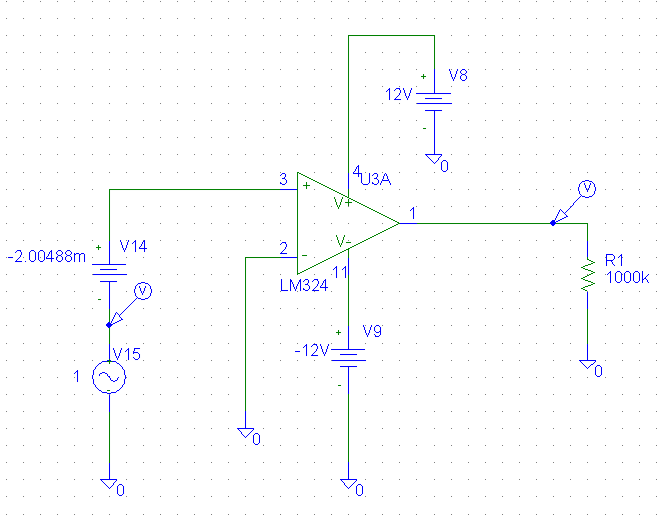
\includegraphics[width=\textwidth]{fig/1_schaltung.png}
	\caption{Schaltung zur Ermittlung des Frequenzgangs der Leerlaufverst"arkung}
	\label{fig:1_schaltung}
\end{figure}

\begin{figure}%[h!]
	\centering
	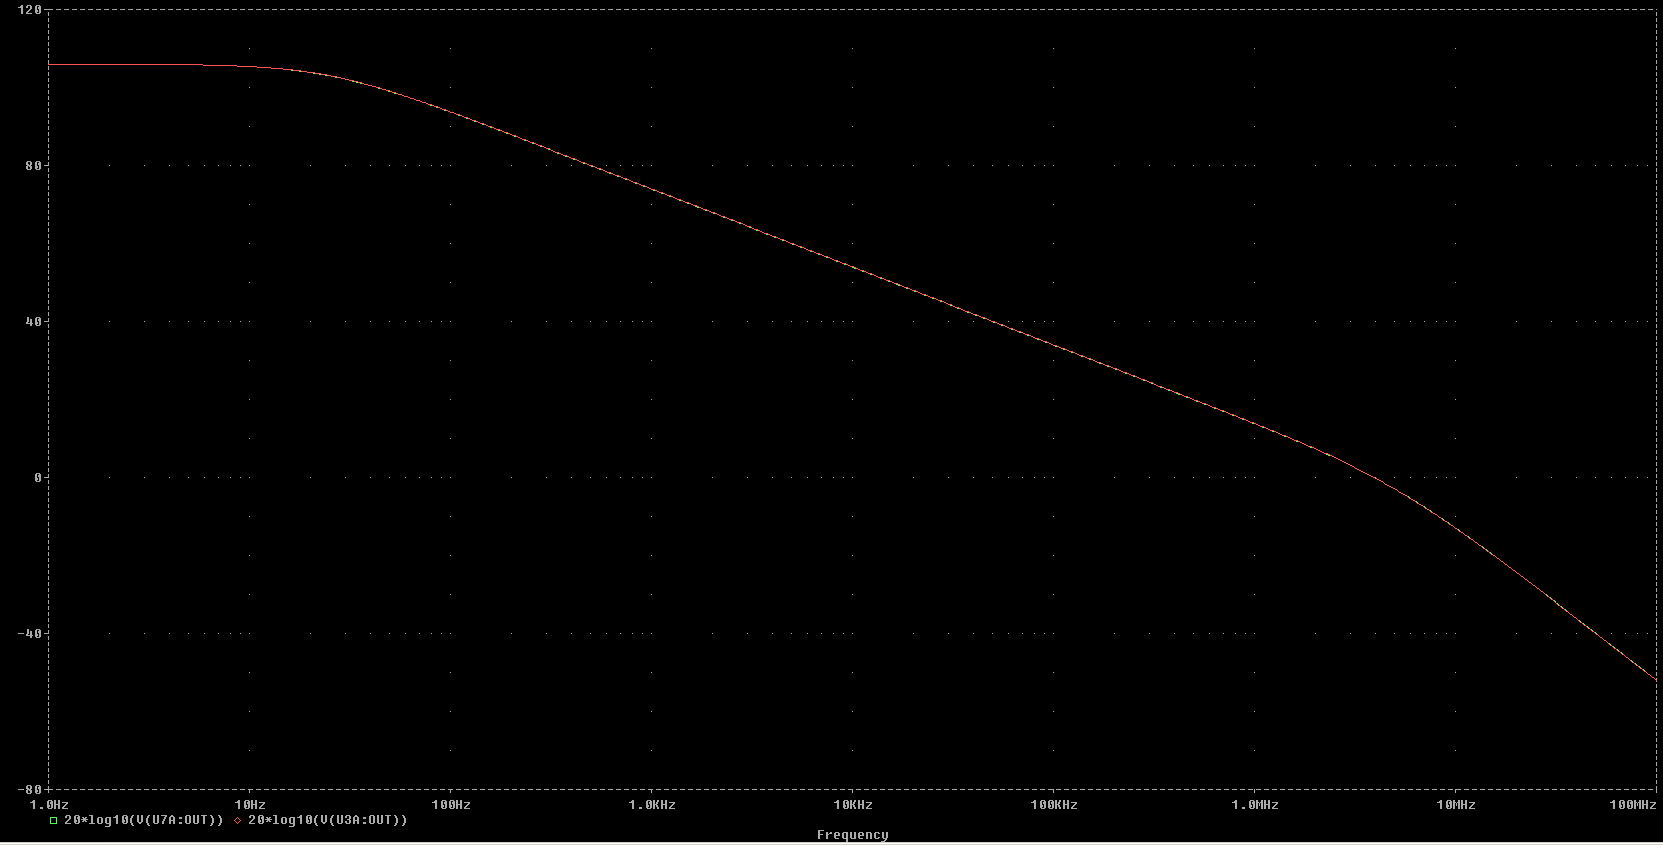
\includegraphics[width=\textwidth]{fig/1_bode.png}
	\caption{Vergleich der Bodediagramme des Makromodells und des ABM-Modells}
	\label{fig:1_bode}
\end{figure}




\section{Beispiel 2: Z"ahler}

Der Z"ahler besitzt die folgende Z"ahlabfolge:

$F_H$, $E_H$, $D_H$, $C_H$, $B_H$, $4_H$, $3_H$, $2_H$, $1_H$, $0_H$, $F_H$, ...

Die maximale Taktrate mit der die Schaltung betrieben werden kann betr"agt 16.12 MHz.

Wird diese Taktrate "uberschritten, so treten beim Timing Mode ``Maximum'' mehrere Warnungen in der Simulation auf.
Diese zeigen, dass gewisse Zeiten der Flip-Flops nicht eingehalten werden.

\section{Beispiel 3: Charge Balancer}

Die gegebene Schaltung wurde durch folgende Elemente erweitert:

\begin{itemize}
 \item ein 4-bit Synchronz"ahler U2 (74293), der den Takt des D-Flipflops verwendet und durchgehend von 0 bis 15 z"ahlt (der Z"ahler l"auft dann "uber und beginnt wieder bei 0)
 \item ein 4-bit Synchronz"ahler U3 (74293), der den Ausgang des NAND-Gatters als Takt verwendet und so die Impulse der Schaltung z"ahlt
 \item ein 4-bit Latch U4 (74176), das jedes Mal beim Erreichen des letzten Taktes von U2 (Z"ahlerstand 15) den aktuellen Z"ahlerstand von U3 speichert
 \item Logik, die beim Erreichen des letzten Taktschritts in der positiven H"alfte des Takts das Latch U4 l"adt
 \item Logik, die beim Erreichen des letzten Taktschritts in der negativen H"alfte des Takts den Z"ahler U3 zur"ucksetzt
\end{itemize}

\begin{figure}[ht]
 \centering
 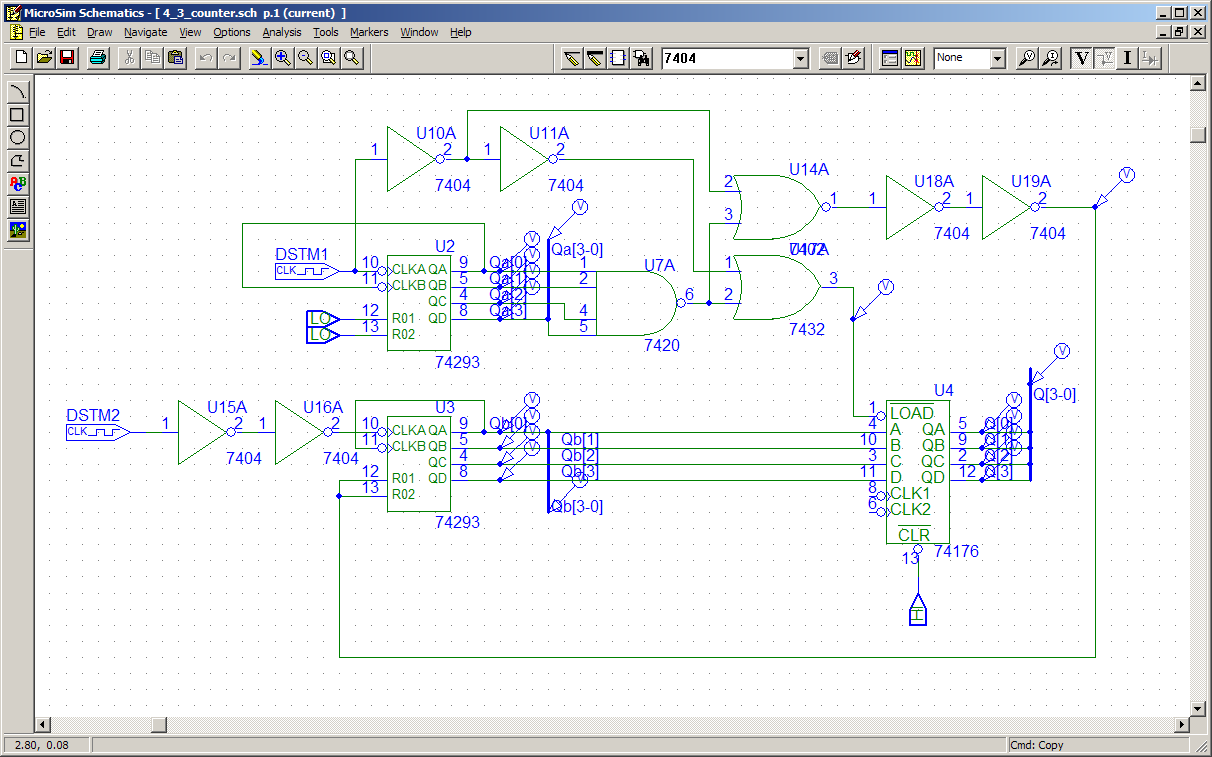
\includegraphics[width=\textwidth]{./img/4_3_counter_schem.PNG}
 \caption{Z"ahler f"ur Beispiel 3}
 \label{fig:4_3_counter_schem}
\end{figure}


Diese Erweiterungen wurden zuerst seperat simuliert (siehe Abbildung~\ref{fig:4_3_counter_schem}). Dabei muss besonders darauf geachtet werden, dass sich durch die Propagation Delays die Signale nicht so verschieben, dass es zu undefinierten Zust"anden kommt. Erreicht wurde das durch eine zus"atzliche Verz"ogerung durch 2 hintereinandergeschaltene Inverter.

Abbildung~\ref{fig:4_3_counter} stellt die Funtionsweise der Schaltung dar. U2 z"ahlt immer von 0 bis 15, U3 z"ahlt mit einem anderen Takt hoch. Erreicht U2 den Wert 15, wird der Wert von U3 im Latch U4 gespeichert und U3 zur"uckgesetzt.

\begin{figure}[ht]
 \centering
 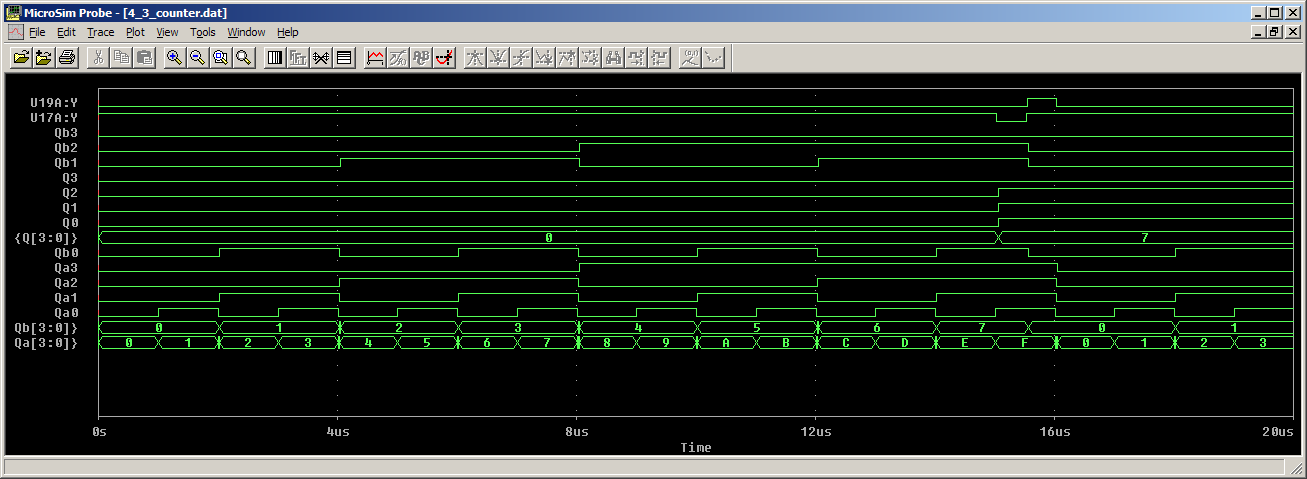
\includegraphics[width=\textwidth]{./img/4_3_counter.PNG}
 \caption{Simulation des Z"ahlers f"ur Beispiel 3}
 \label{fig:4_3_counter}
\end{figure}

Die Schaltung wurde dem gegebenen Charge Balancer hinzugef"ugt und wiederum getestet (siehe Abbildung~\ref{fig:4_3_schem}). Wegen leicht verschobenen Takt- und Signalflanken mussten wieder 2 Inverter hinzugef"ugt werden. Die Simulation mit typischen Timings funktionierte (siehe Abbildung~\ref{fig:4_3}), das Springen des Ausgangswerts ist darauf zur"uckzuf"uhren, dass die Impulse nicht genau zu jedem 16. Takt auftreten, und deswegen pro Periode von 16 Takten ein Takt mehr oder weniger aufgenommen werden kann (dieser Fall tritt jedoch nur selten und nur eine Periode lang auf). Au\ss{}erdem erkennt man die Einschwingphase der Schaltung.

\begin{figure}[ht]
 \centering
 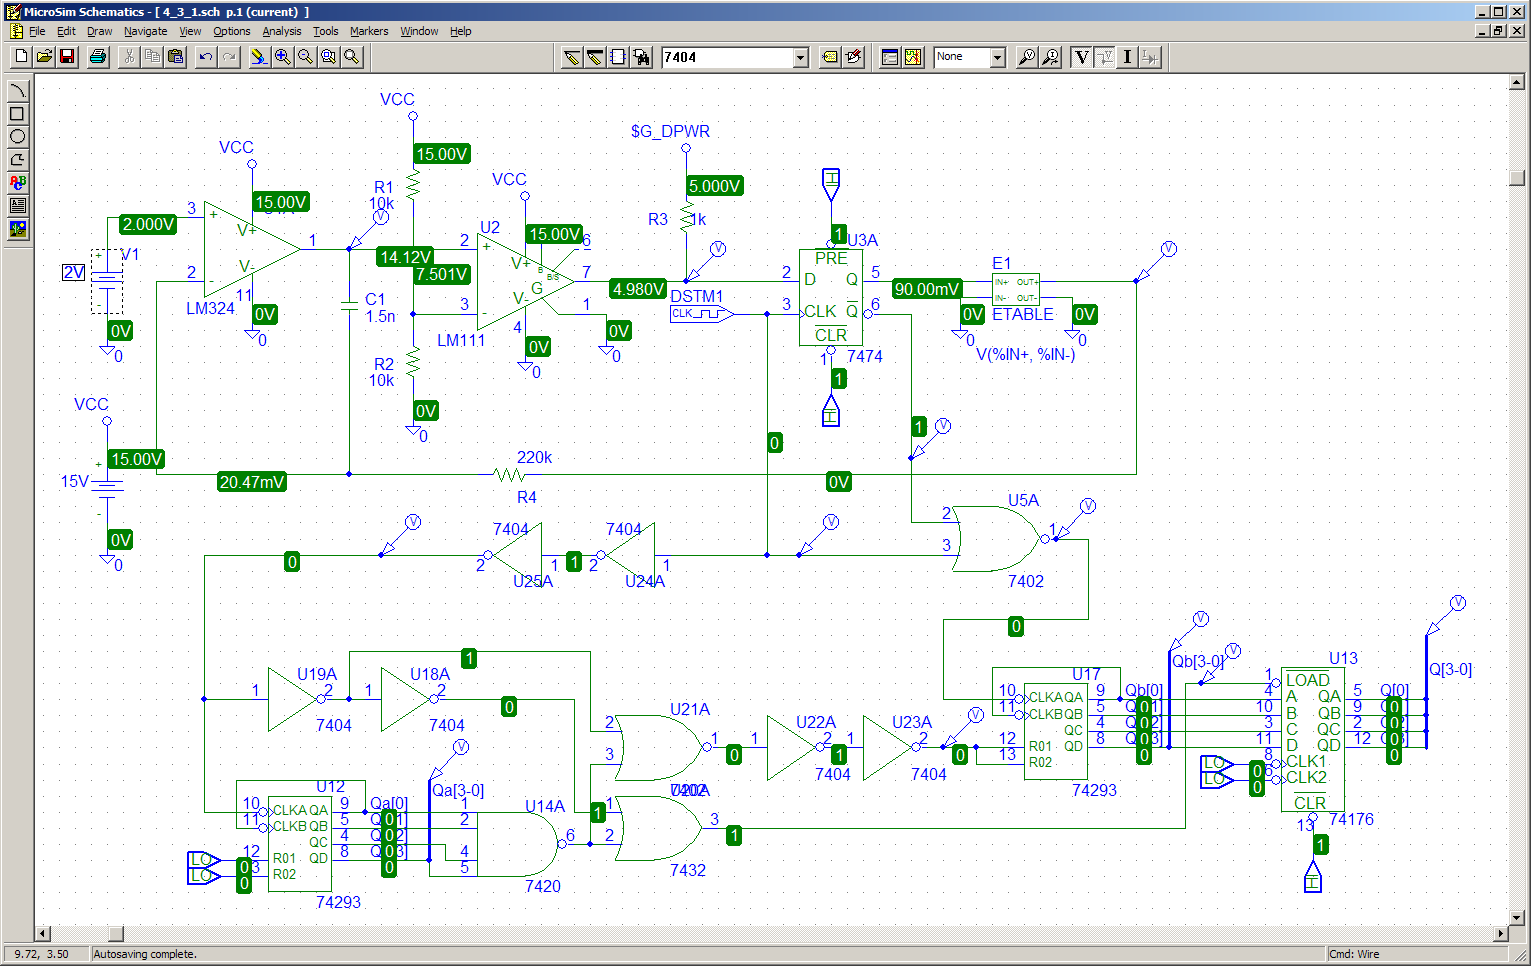
\includegraphics[width=\textwidth]{./img/4_3_schem.PNG}
 \caption{Vollst"andige Schaltung f"ur Beispiel 3}
 \label{fig:4_3_schem}
\end{figure}

\begin{figure}[ht]
 \centering
 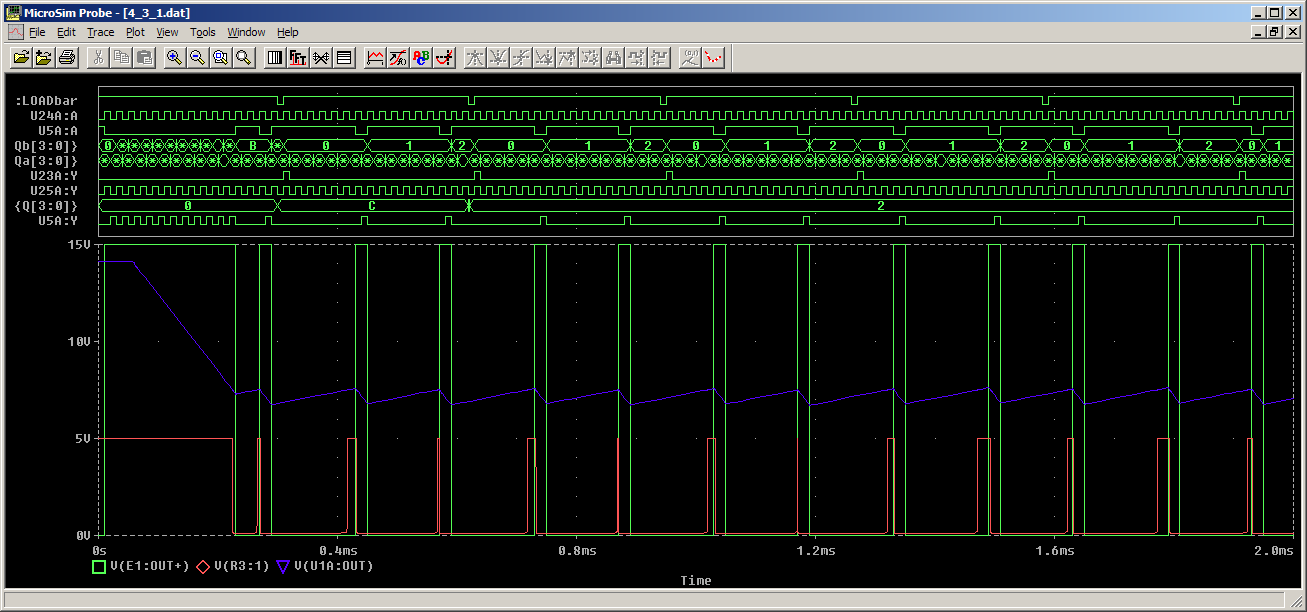
\includegraphics[width=\textwidth]{./img/4_3.PNG}
 \caption{Simulation der vollst"andigen Schaltung f"ur Beispiel 3}
 \label{fig:4_3}
\end{figure}

Bei der Worst-Case-Simulation funktionierte die Schaltung "uberhaupt nicht mehr, da die Takt- und Signalimpulse oft so stark versetzt waren, dass es zu undefinierten Zust"anden kam. Auch durch l"angeres Herumprobieren und Umbauen der Schaltung verbesserte sich die Situation nicht.


\clearpage
\section{Beispiel 4: Temperaturabh"angige L"uftersteuerung}

Passend zu den hohen Temperaturen wurde als letztes Beispiel eine L"uftersteuerung entworfen und simuliert, die aus der aktuellen Temperatur, gemessen mit einer Diode, ein PWM-Signal erzeugt, mit dem "uber einen MOSFET ein L"ufter angesteuert werden kann.

\begin{figure}[ht]
 \centering
 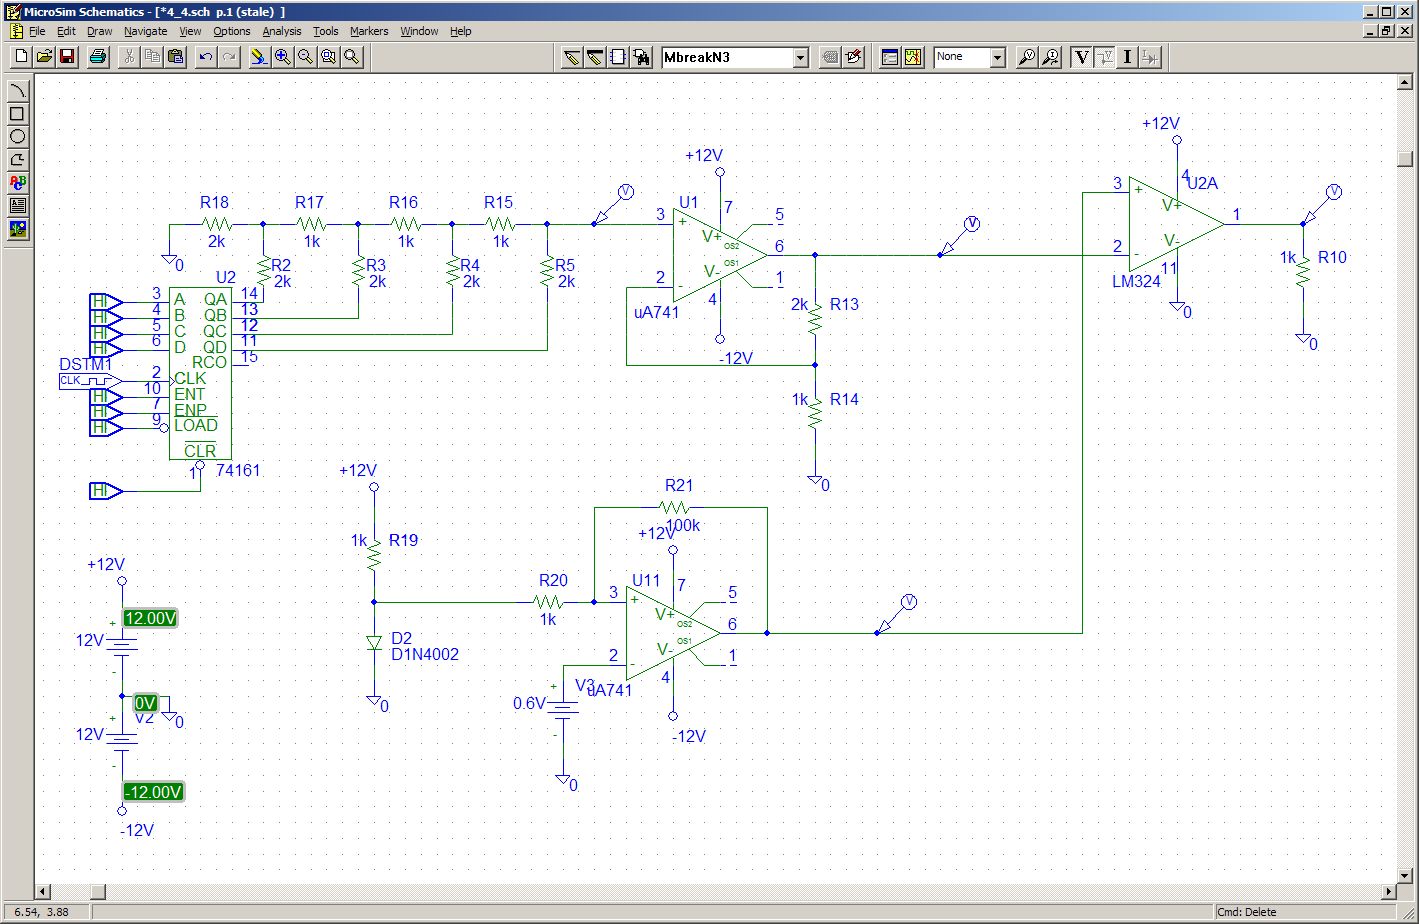
\includegraphics[width=\textwidth]{./img/4_4_schem.PNG}
 \caption{Schaltung der L"uftersteuerung}
 \label{fig:4_4_schem}
\end{figure}

Zu erst muss aus der Ausgangsspannung der Diode eine absolute Temperatur errechnet werden. Ausgenutzt wurde die "Anderung der Diodenflussspannung von $-1.7\frac{mV}{K}$. Mit einem invertierenden Verst"arker wurde die Flussspannung der Diode (durch Simulation ermittelt, ca. 0.6V) subtrahiert und die "Anderung der Flussspannung auf brauchbare Werte verst"arkt (siehe Abbildung~\ref{fig:4_4_schem}). Der Offset und die Verst"arkung k"onnen so berechnet werden, dass sich im Temperaturbereich von 20 bis 40 Grad Celsius eine Spannung von 0V bis 10V ergibt.

F"ur die Erzeugung der PWM wurde mit Hilfe eines Z"ahlers ein Rampensignal erzeugt. Ein 4-bit Synchronz"ahler (74293) z"ahlt immer wieder von 0 bis 15 und l"auft dann wieder "uber. Am Ausgang des Z"ahlers befindet sich eine Widerstandsleiter, durch die eine analoge Spannung zwischen 0 und 5V erzeugt wird. Diese Spannung ist s"agezahnf"ormig. Mit einem nichtinvertierenden Verst"arker wird diese Spannung dann an den gew"unschten Bereich angepasst.

Ein Komparator vergleicht die S"agezahnspannung und die Temperaturspannung. Je nach H"ohe der Temperaturspannung schaltet der Komparator um, sobald die Rampe die Temperaturspannung "uberschreitet. Dadurch ist die high-Dauer des Komparatorausgangs je l"anger, umso h"oher die Temperaturspannung ist. Abbildung~\ref{fig:4_4_2V} zeigt das Verhalten der Schaltung bei einer niedrigen Temperatur, Abbildung~\ref{fig:4_4_7V} zeigt das Verhalten bei einer h"oheren Temperatur. Am Ausgang k"onnte sich ein n-Kanal MOSFET befinden, der in dieser Zeit einen L"ufter einschaltet. Dadurch ergibt sich eine einfache Temperatursteuerung, die die L"ufterdrehzahl an die Temperatur anpasst.

\begin{figure}[ht]
 \centering
 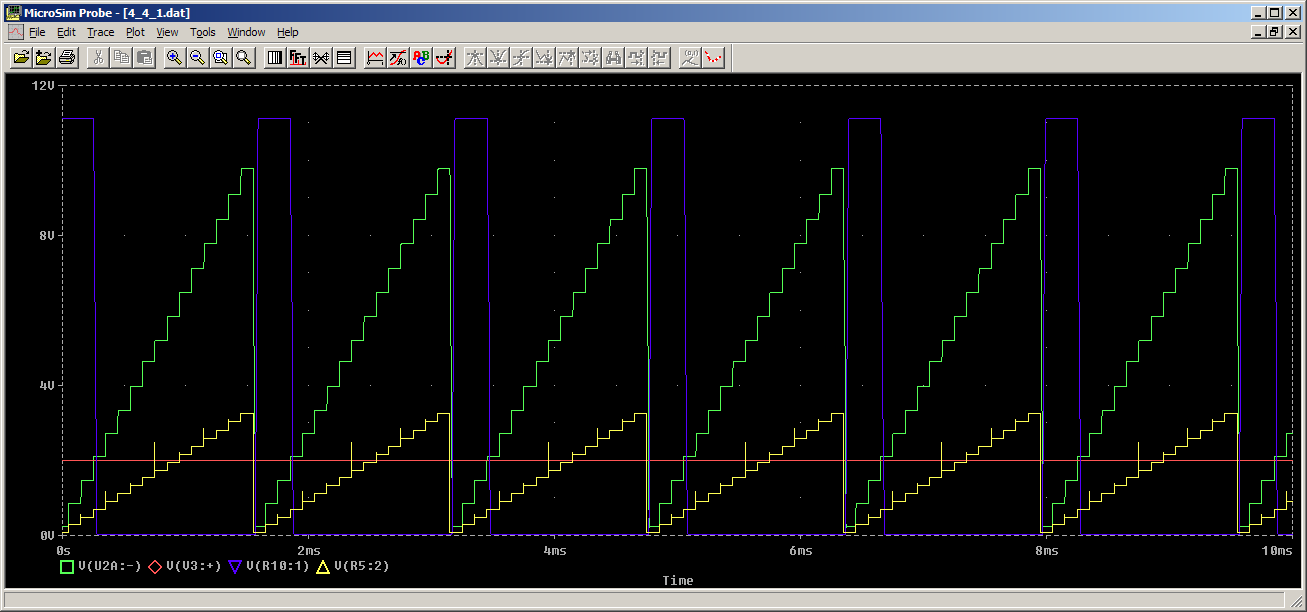
\includegraphics[width=\textwidth]{./img/4_4_2V.PNG}
 \caption{Verhalten der L"uftersteuerung f"ur eine Temperaturspannung von 2V}
 \label{fig:4_4_2V}
\end{figure}

\begin{figure}[ht]
 \centering
 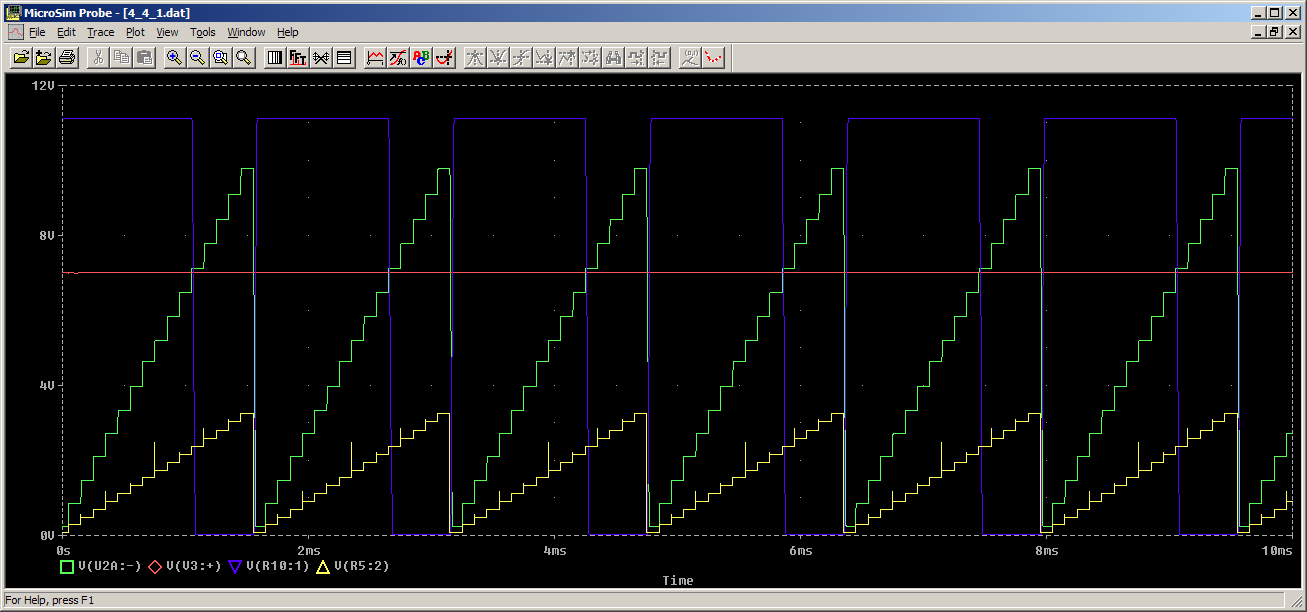
\includegraphics[width=\textwidth]{./img/4_4_7V.PNG}
 \caption{Verhalten der L"uftersteuerung f"ur eine Temperaturspannung von 7V}
 \label{fig:4_4_7V}
\end{figure}

Leider konnten wir die gesamte Schaltung nicht mit der verwendeten Version von PSpice simulieren, da die Anzahl der Nodes zu hoch f"ur die Studentenversion war. Deswegen wurde nur eine vereinfachte Version simuliert, bei der die Erzeugung einer Temperaturspannung durch eine Spannungsquelle ersetzt wurde (siehe Abbildung~\ref{fig:4_4_1_schem}).

\begin{figure}[ht]
 \centering
 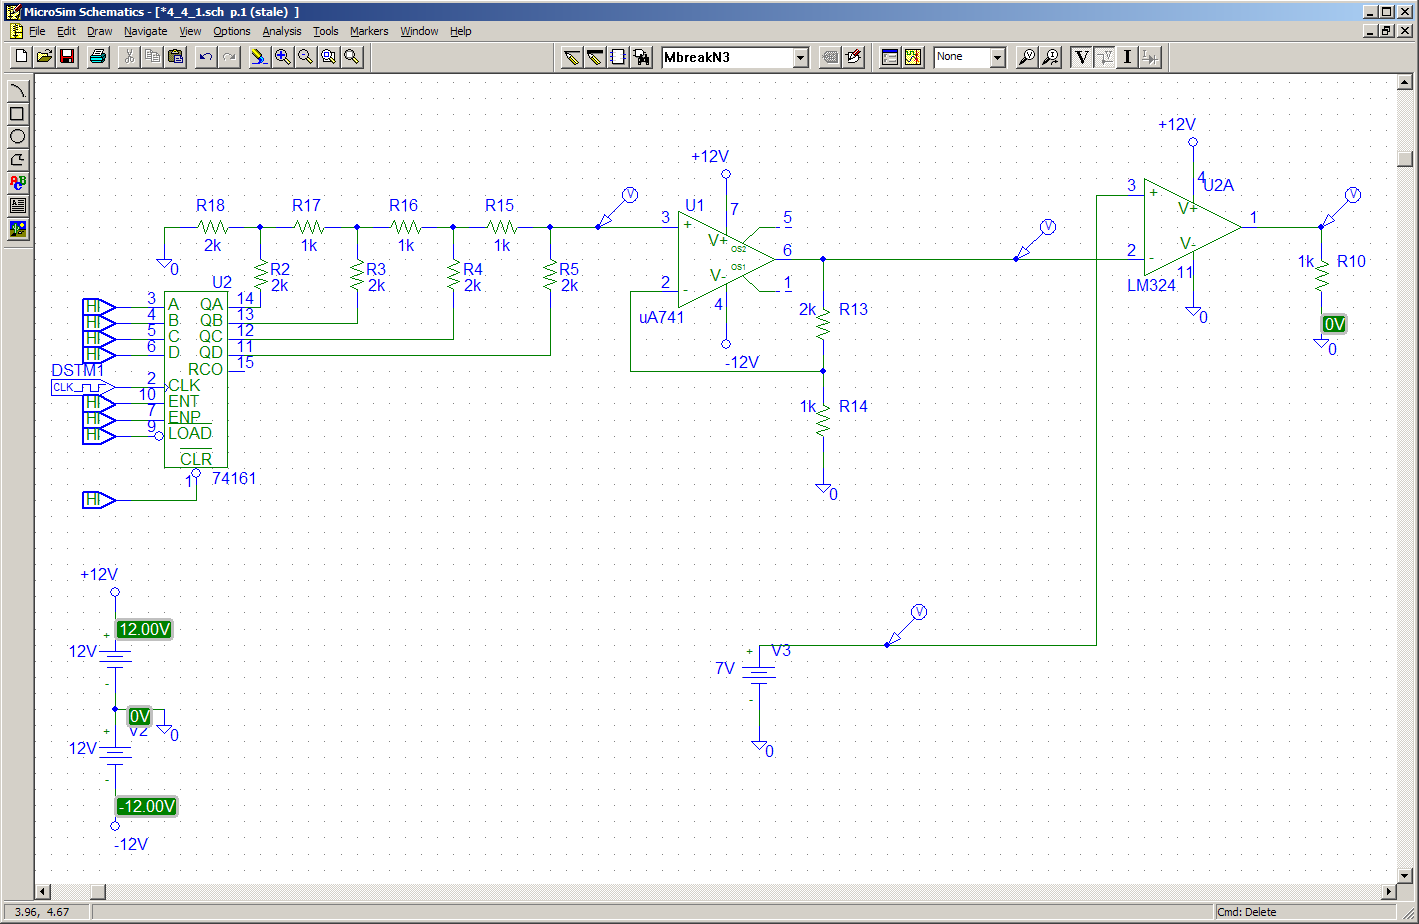
\includegraphics[width=\textwidth]{./img/4_4_1_schem.PNG}
 \caption{Vereinfachte Schaltung zur Simulation mit PSpice}
 \label{fig:4_4_1_schem}
\end{figure}



% \newpage
% 
% \chapter{Listings}
% 
% \section{Simulation}
% \lstinputlisting[language=matlab]{bla}

%\section{Noise Cancelation}
%\lstinputlisting[language=matlab]{../matlab/3_4/m34.m}

%\section{Performancevergleich (N)LMS}
%\lstinputlisting[language=matlab]{../implementation/lms_performance.m}


% **************************************************************************************************
% **************************************************************************************************

%\appendix
%\bibliographystyle{/.base/ieeetran}
%\bibliography{_bibliography}

% place all floats and create label on last page
\FloatBarrier\label{end-of-document}
\end{document}

